This \cgal\ package provides functions to compute global informations
on the shape of a set of 2D or 3D objects such as points. It provides the computation of axis-aligned bounding boxes, centroids of point sets, barycenters of weighted point sets, as well as linear least squares fitting for point sets in 2D, and point sets as well as triangle sets in 3D. The sets are specified by iterator ranges of containers.\\

\begin{center}
    \label{fit}
    % Image
    \begin{ccTexOnly}
      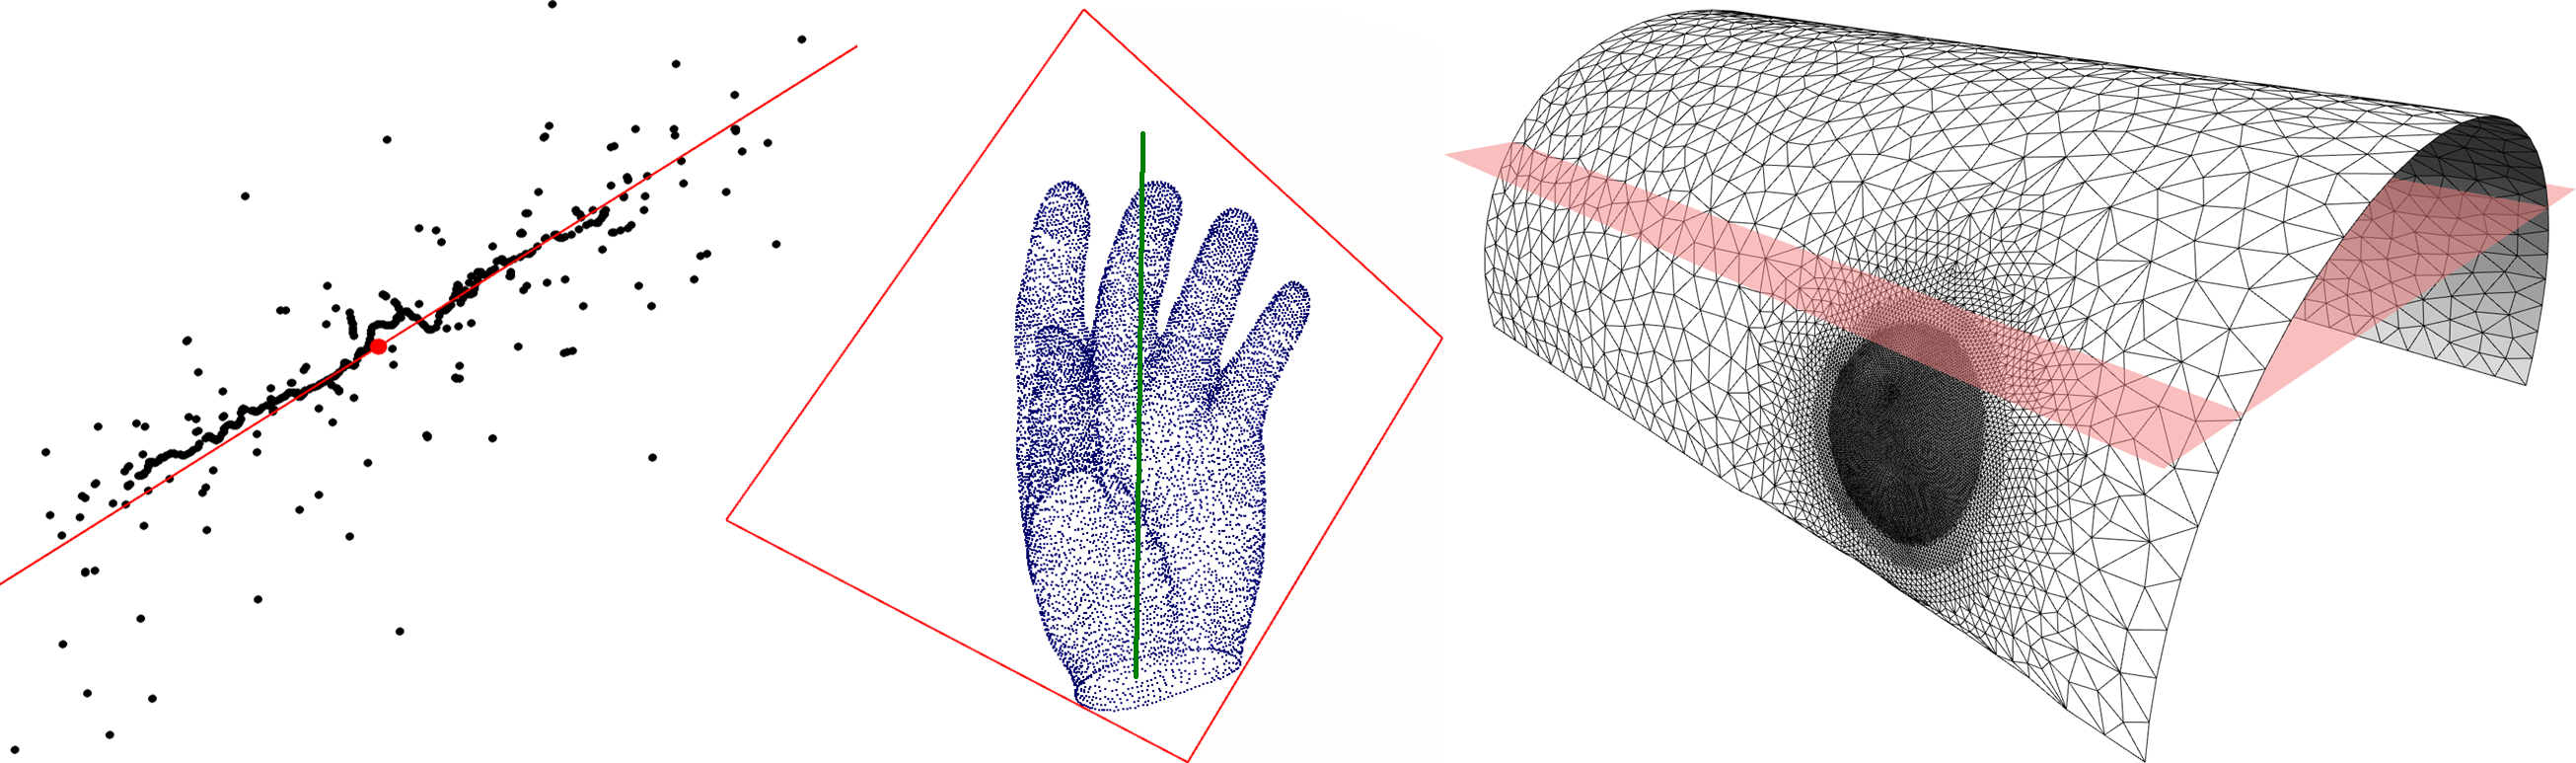
\includegraphics[width=1.0\textwidth]{Principal_component_analysis/fit}
    \end{ccTexOnly}
    \begin{ccHtmlOnly}
        <img width="100%" border=0 src="./fit.png"><P>
    \end{ccHtmlOnly}
    % Title
    \begin{figure}[h]
        \caption{Left: fitting a line to a 2D point set.
                 Right: fitting a line and a plane to a 3D point set.}
    \end{figure}
\end{center}

